\documentclass[10pt,preprint]{sigplanconf}

\usepackage{times}
\usepackage{graphicx}
\usepackage{datetime}
\usepackage{url}
\usepackage{hyperref}


%\conferenceinfo{}{}
%\copyrightyear{} 

%\date{}

\authorinfo{}{Department of Computer Science, University of California, Irvine}

\begin{document}

\title{GraphDTC: A Graph Processing System for Scalable and Precise Program Analysis} 
\maketitle


\begin{abstract}
In this technical report, we present a graph processing system, Graph-DTC. It is designed to efficiently compute dynamic transitive closure (DTC) on program graphs of large complex systems (e.g. Linux), which may be of the order of a billion vertices, using a single machine. DTC computation enables us to get precise software diagnostics such as bugs and data flow information. Thomas Reps first showed in his seminal work how graph reachability problems like the DTC problem could aid different program analysis techniques. 

While the DTC problem has been studied for more than two decades, implementing it on large graphs has not been scalable. As a result, most existing program analysis and bug detection techniques have been deprived of detailed program information (e.g. precise aliasing information), which has limited their highest attainable precision. In order to leverage those techniques, we introduce a novel graph computation model, the edge-pair centric model, on which we build GraphDTC. GraphDTC enables those techniques to capture more detailed information about the software, and thus produce more precise diagnostics information. 
\end{abstract}


\section{Introduction}

Static program analysis techniques such as alias/points-to analysis, flow/path-sensitive analysis, context-sensitive analysis, and object-sensitive analysis have been extensively used for revealing various diagnostic information of software programs~\cite{Xu}. For instance, alias analysis, a technique for determining pointers that point to the same location~\cite{alias}, has been used to discover the presence of certain kinds of faults in Linux and OpenBSD kernels~\cite{Chou, Palix}. Another example is the work of Bugrara and Aiken~\cite{aiken08} who checked for security vulnerabilities in Linux, using path- and context-sensitive analyses, two subtypes of alias analysis. They extracted unchecked user pointer dereferences in Linux to prevent the exposure of the kernel space. More recently, alias analysis have also been used to identify resource leaks~\cite{manu}.

Despite their success in various important applications, most of these static program analysis techniques had to grapple with one major challenge: how to balance the trade-off between (1) the precision of their outcomes (e.g. false negatives in bug detection) and (2) their efficiency. 

The precision of these techniques depends on the comprehensiveness of the information used by them. For example, context-sensitive analysis uses information about the calling context of program method calls, whereas context-insensitive analysis does not~\cite{Xu}. Similarly, flow-sensitive analysis considers the flow of the program and thus yields separate solutions for each ordering of the program points, whereas flow-insensitive analysis ignores flow information and yields an approximated solution that holds for all orderings of program points in a program~\cite{hardekopf}.

Unfortunately, greater precision comes with a cost on efficiency. As a result, the scalability of precise analysis techniques have been restricted. For instance, context-sensitive analysis based techniques have been shown to scale to hundreds of thousands of lines~\cite{aiken06, liang04}, path-sensitive
to tens of thousands of lines~\cite{aiken06, wilson}. Alternately, alias analyses that scale to a million lines of code have been found to give imprecise alias information with respect to the actual aliasing when the code is executed~\cite{aiken06, liang, mock}. 

To address this precision-efficiency bottleneck, researchers have used program abstraction in order to keep only information that is relevant for proving properties of interest~\cite{zhang}. Such approaches have an overhead of computing the abstractions. Other researchers have addressed the scalability problem by simply ignoring intra-procedural analysis and by only analyzing procedures independently (e.g.~\cite{aiken08}).

In this work, we tackle the problem head-on, by providing an infrastructure that can provide the large scale computation that precise program analysis techniques need for both intra-procedural and even inter-procedural analysis. We design a graph processing system that can be used to perform computations over massive program graphs (e.g. call graphs) which are used by such techniques. Our inspiration comes from the insights of Thomas Reps~\cite{reps}.

Reps shows that program analysis problems could be transformed to graph reachability problems. In particular, he shows how program analysis problems could be reduced to a CFL (Context-Free Language)-reachability problem, which is a type of a \textit{transitive closure (TC)} problem. The TC problem is to determine paths, or connected edges, in a directed graph. In the \textit{CFL-reachability problem}, a path is considered to connect two nodes only if the concatenation of the labels on the edges of the path is a word in a particular context-free language~\cite{reps}. In order to solve the CFL-reachability problem in a directed graph with labels, we need to iteratively add an edge each time we find such a path, such that the edge connects the end vertices of the path. Solving the CFL-reachability problem can thus be essentially reduced to computing the \textit{dynamic transitive closure (DTC)} of a directed graph.  

Our graph processing system, GraphDTC, can efficiently compute the DTC on graphs of the order of a billion edges, on a single machine. With such a system, we can facilitate the use of the aforementioned precise program analysis techniques and thus enable them to extract more precise diagnostics information. (An elaborate plan for gathering such information is given towards the end of this report.) Although there are other approaches for scaling program analysis, such as~\cite{db-backed} and~\cite{hardekopf} our approach is significantly different and novel. We offer a systems solution to a bottleneck in software analysis, by addressing a fundamental problem in programming language design, the CFL-reachability problem. 

The rest of this technical report is organized as follows: Section~\ref{sec:gdtccompmod} presents the fundamental computation model of GraphDTC. Section~\ref{sec:design} provides the design and implementation of our system. Then in Section~\ref{sec:evpln}, the evaluation plan for GraphDTC is presented. Finally, we conclude the report in Section~\ref{sec:cncl}. 
 
%\section{Preliminaries}
\label{sec:prelim} 

\section{GraphDTC Computation Model}
\label{sec:gdtccompmod}

In this section, we present the GraphDTC computation model. In~\ref{subsec:epcm}, we present a novel edge-pair centric (EPC) model that can be used to address the DTC computation on a directed, labelled graph. Finally we present the edge computation model which is built on the EPC model in~\ref{subsec:ecm}.

%In~\ref{subsec:prob}, we emphasize upon our main dynamic transitive closure problem.
%\subsection{Problem}
%\label{subsec:prob}

\subsection{Edge-Pair Centric (EPC) Model}
\label{subsec:epcm}

\begin{figure}[!htbp]
	\begin{center}
		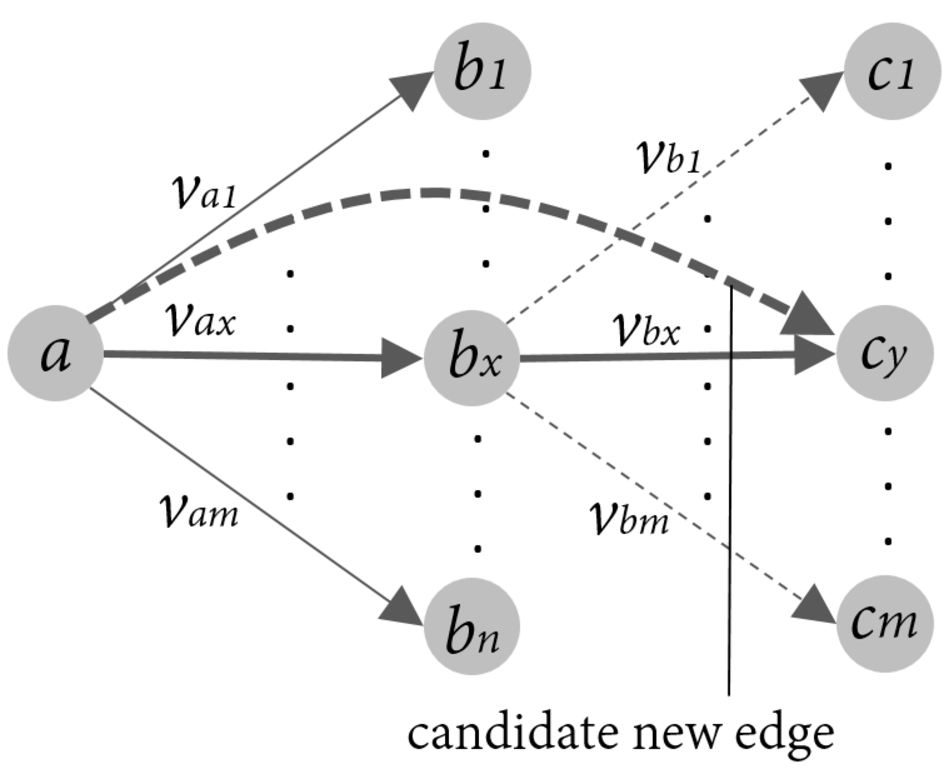
\includegraphics[scale=0.35]{Figures/epcmodel.pdf}
	\end{center}
	\caption{The Edge-Pair Centric (EPC) model.}
	\label{fig-epcmodel}
\end{figure}

The \textit{EPC model} allows us to (1) find whether there exists a transitive relation between the source and sink vertices in a path of two directed edges and (2) add an edge from the source vertex to the sink vertex if such a relation exists, while ensuring that the ``new'' edge does not already exist.  

Fig.~\ref{fig-epcmodel} demonstrates the use of the EPC model. It shows all the out-edges of two vertices $a$ and $b_x$ in an arbitrary graph. We want to find whether there exists a transitive relation from $a$ to $c_y$, and add a directed edge from $a$ to $c_y$ if the relation does exist. (The reason why $b_x$'s other out-edges have been dashed will be explained shortly). The bold dashed edge shows the candidate new edge. If the symbols represented by the edge values, $v_{a_x}$, $v_{b_x}$ form a valid production, in the sequence shown, then a transitive relation exists between vertices $a$ and $c_y$. In that case, all out-edges of $a$ are scanned to check whether directed edge $(a,c_y)$ already exists. If not, the edge is added. 

As can be seen, to check for transitive closure between source $a$ and sink $c_y$, we do not require to check out-edges of the mid-vertex $b_x$. These edges do not belong to the EPC model and have thus been shown as dashed.      

\subsection{Edge Computation Model}
\label{subsec:ecm}

\begin{figure*}[!htbp]
	\begin{center}
		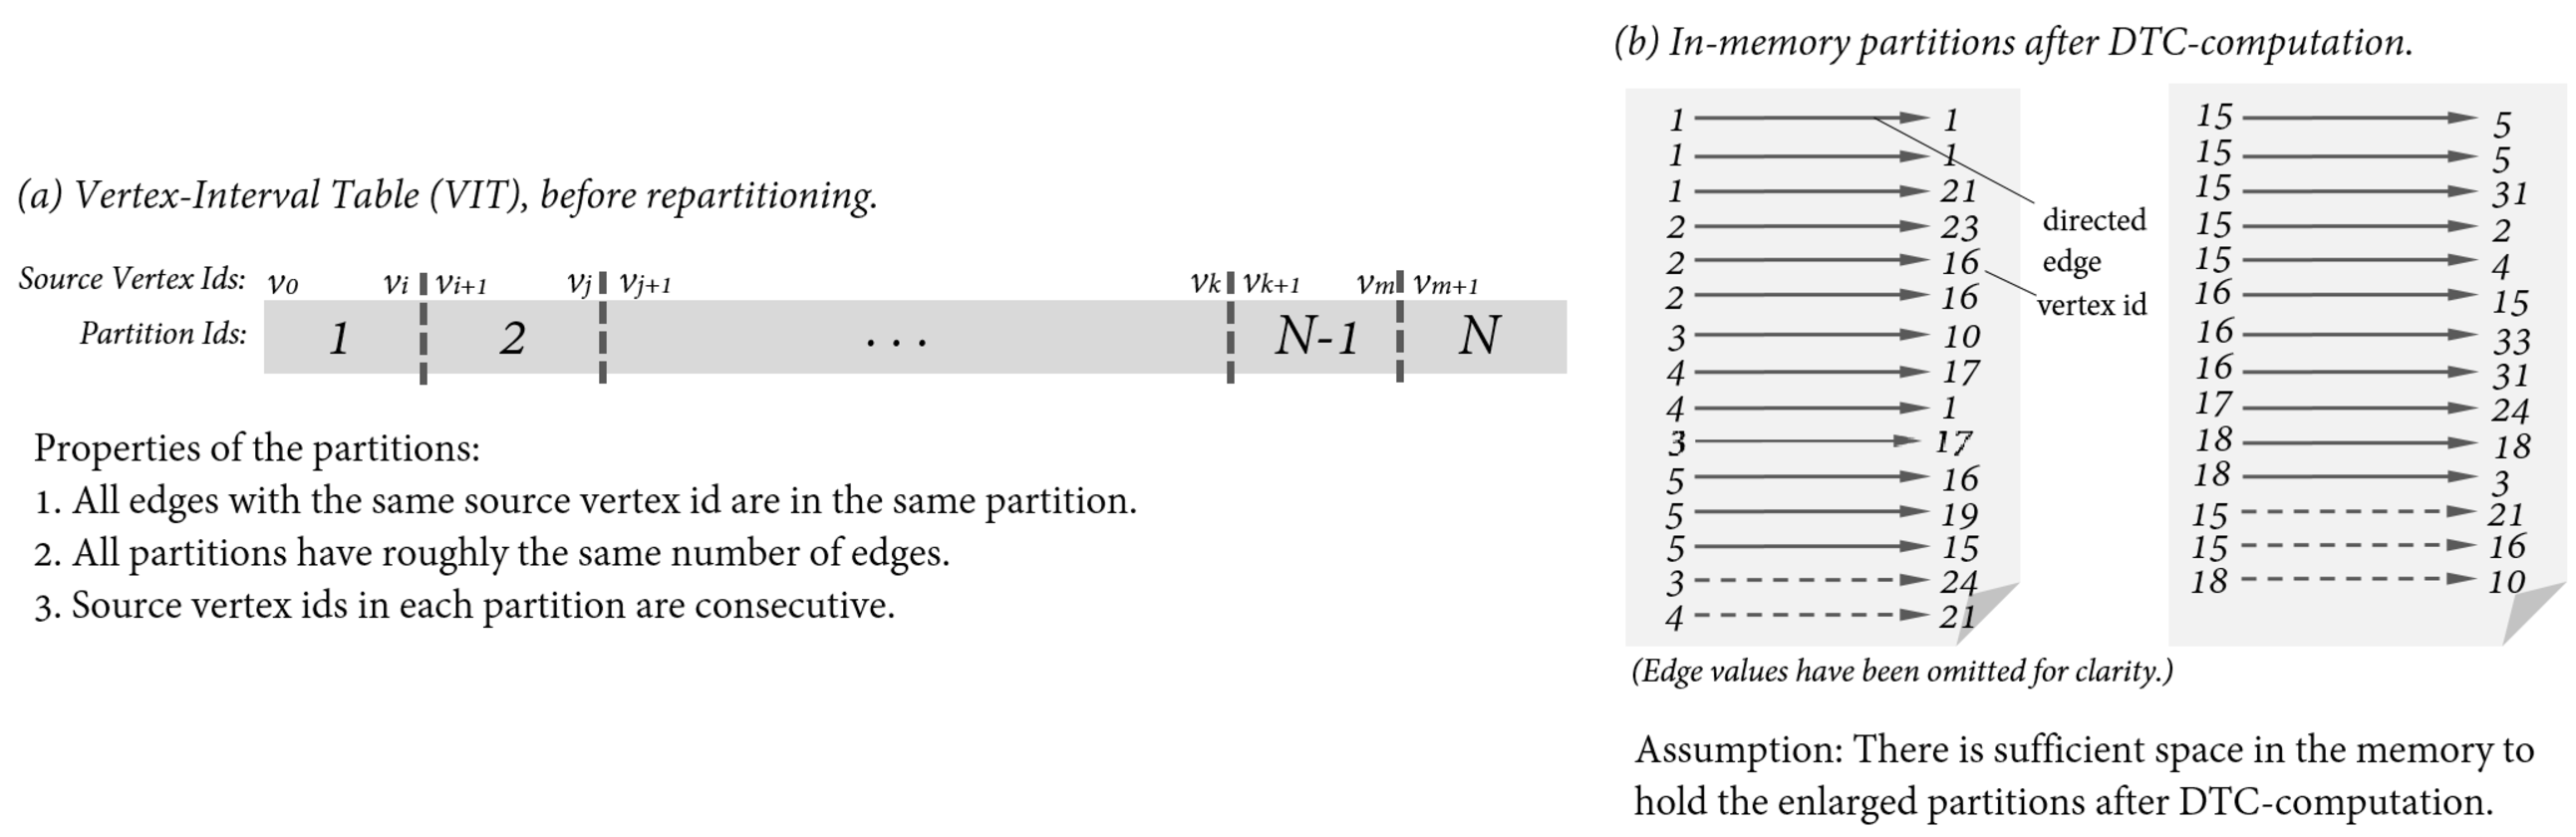
\includegraphics[scale=0.4]{Figures/dtccompmodel.pdf}
	\end{center}
	\caption{DTC computation model.}
	\label{fig-dtccompmodel}
\end{figure*}

Fig.~\ref{fig-dtccompmodel}, shows the DTC computation model of GraphDTC. In preprocessing, which will be shown in~\ref{subsec:pp}, partitions from the input graph are generated by allocating vertices to intervals, creating a vertex-interval table, as shown in Fig.~\ref{fig-dtccompmodel}(a). The conditions for creating the partitions are also shown in the figure. Fig.~\ref{fig-dtccompmodel}(b) shows an example of two partitions on which DTC computation has been done in the memory. In this example, we have omitted edge values. The edges with dashed arrows are new edges generated as a result of the computation. For instance, edge $(4, 21)$ was generated as a result of the edges $(4, 1)$ and $(1, 21)$. 

%\subsection{Alternate Techniques}
\label{subsec:alt}

\section{System Design and Implementation}
\label{sec:design}

In this section, we discuss the design and implementation of all the phases of GraphDTC. We have implemented GraphDTC in Java. The system has been written in approximately 4,000 lines of code (LOC). 

Fig.~\ref{fig-ppphase} shows the preprocessing phase of Graph DTC. The remaining phases, and the coordination between them, are shown in Fig.~\ref{fig-compphases}. The mechanisms of each phase are explained in the following subsections. 


\begin{figure*}[!htbp]
	\begin{center}
		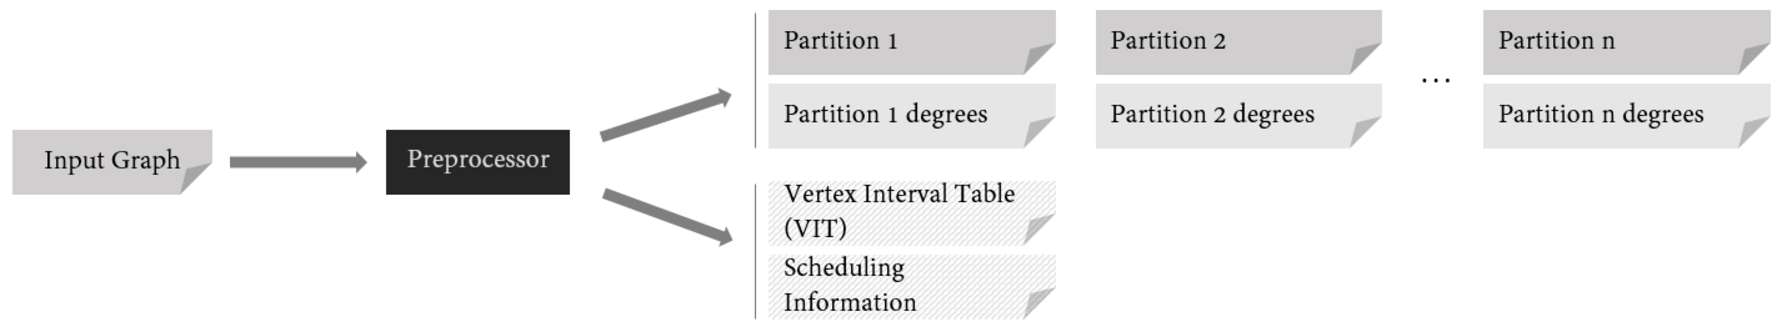
\includegraphics[scale=0.5]{Figures/ppphase.pdf}
	\end{center}
	\caption{GraphDTC preprocessing phase.}
	\label{fig-ppphase}
\end{figure*}

\begin{figure*}[!htbp]
	\begin{center}
		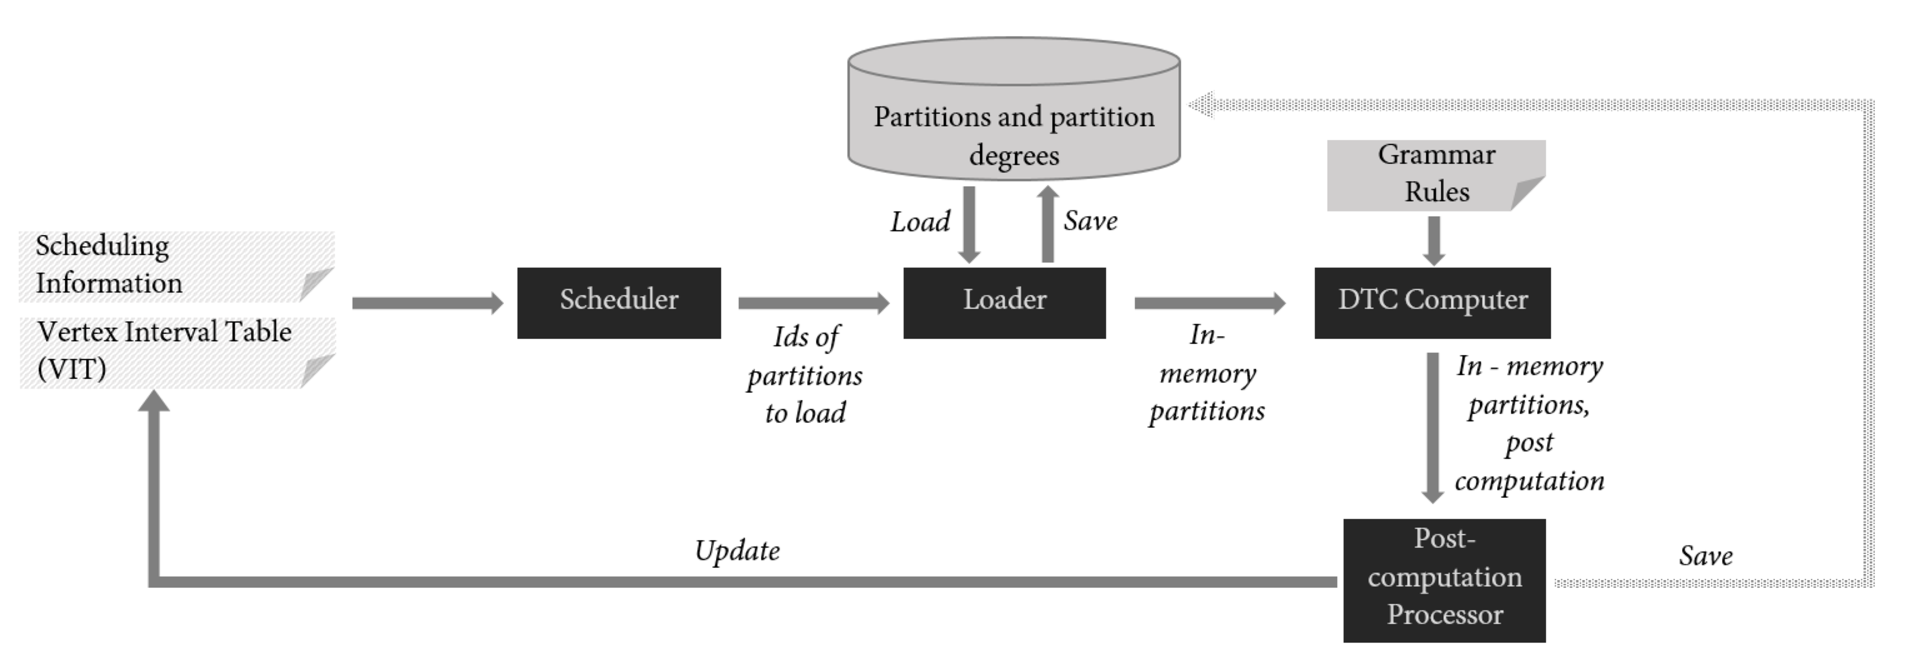
\includegraphics[scale=0.50]{Figures/compphases.pdf}
	\end{center}
	\caption{GraphDTC computation phases.}
	\label{fig-compphases}
\end{figure*}


\subsection{Preprocessing (Partition Generation)}
\label{subsec:pp}

\begin{figure}[!htbp]
	\begin{center}
		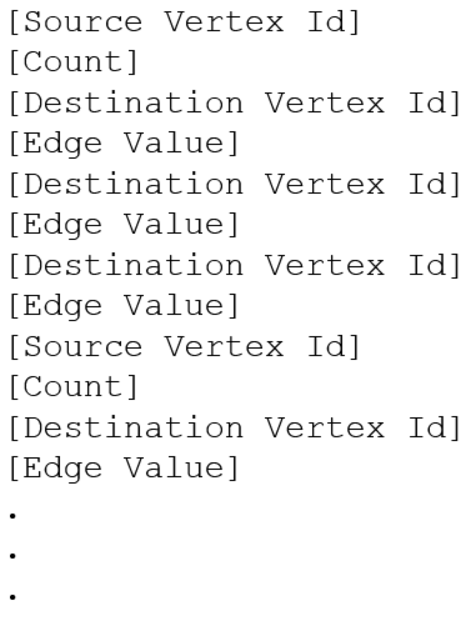
\includegraphics[scale=0.5]{Figures/partfmt.pdf}
	\end{center}
	\caption{Partition data format on disk.}
	\label{fig-partfmt}
\end{figure}

This phase generates partitions by scanning the input graph, which is in an edge list format. In particular, each line of the input graph file has the source vertex id, the destination vertex id, and the edge value. The resultant partition file is stored in a format similar to an adjacency list, as shown in Fig.~\ref{fig-partfmt}. All data are stored in binary in order to reduce the overall size of the partition files.

While generating each partition, the size of each partition should depend on the DRAM memory space for computation, such that at any time the memory can hold two partitions, with just enough space for other meta data structures and system resources. Following this constraint, we can ensure minimal unused memory space during each computation. 

As shown in Fig.~\ref{fig-ppphase}, other products of the preprocessing phase are (1) degrees file for each partition, which is used for setting up the array data structures of a partition when the partition is loaded in the memory, (2) the Vertex-Interval Table (VIT) which is used throughout all phases of GraphDTC to refer to partition information of edges, and (3) the scheduling information, which will be explained in Subsection~\ref{subsec:sch}.

\subsection{Loading Partitions}
\label{subsec:loadingparts}

\begin{figure*}[!htbp]
	\begin{center}
		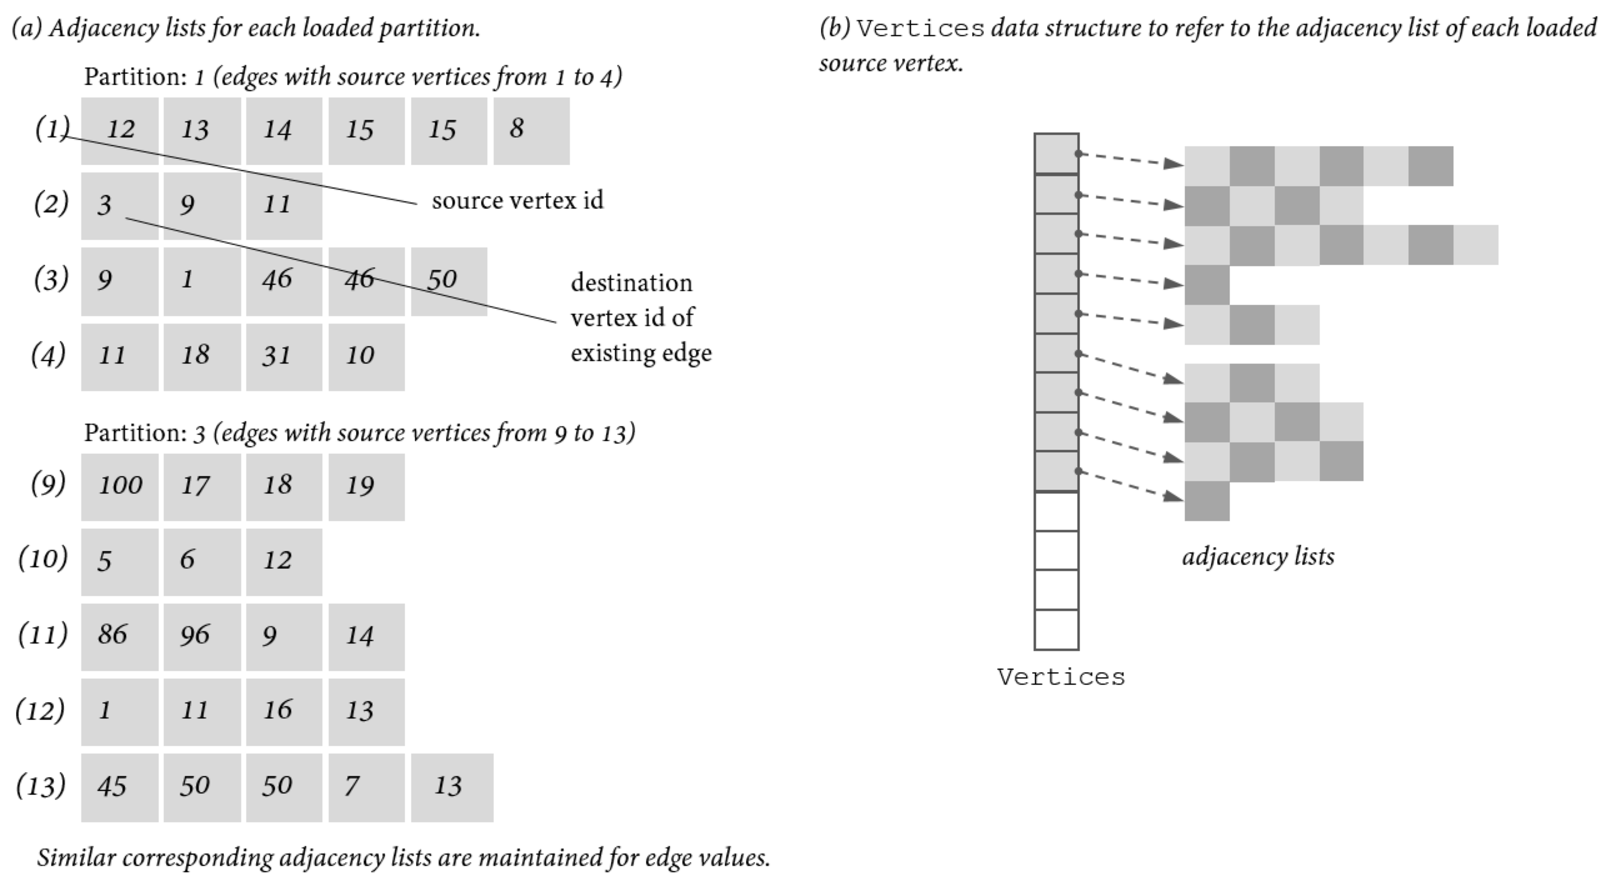
\includegraphics[scale=0.58]{Figures/lddesign.pdf}
	\end{center}
	\caption{Loading design.}
	\label{fig-lddesign}
\end{figure*}

In order to load the partitions in the memory, we use adjacency list data structures via multi-dimensional arrays as shown in Fig.~\ref{fig-lddesign}(a). A data structure, \texttt{Vertices}, is used to refer to the row of each loaded source vertex (Fig.~\ref{fig-lddesign}(b)). \texttt{Vertices} will be useful later when we need to replace only partition in the memory. 

\begin{figure}[!htbp]
	\begin{center}
		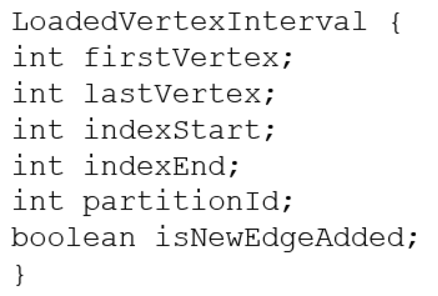
\includegraphics[scale=0.55]{Figures/lvi.pdf}
	\end{center}
	\caption{LoadedVertexInterval data structure for keeping information about partitions loaded in DRAM.}
	\label{fig-lvi}
\end{figure}

Fig.~\ref{fig-lvi} shows another data structure, \texttt{LoadedVertex} \texttt{Interval} that is set-up during loading. As can be seen, it stores the corresponding indexes of the rows of the loaded source vertices in the \texttt{Vertices} data structure. The memory consumption of \texttt{LoadedVertex} \texttt{Interval} is negligible as the total number of partitions is small, and also at most two partitions are loaded in the memory at any time. 

\subsection{Edge Computation}
\label{subsec:edgcomp}

\begin{figure*}[!htbp]
	\begin{center}
		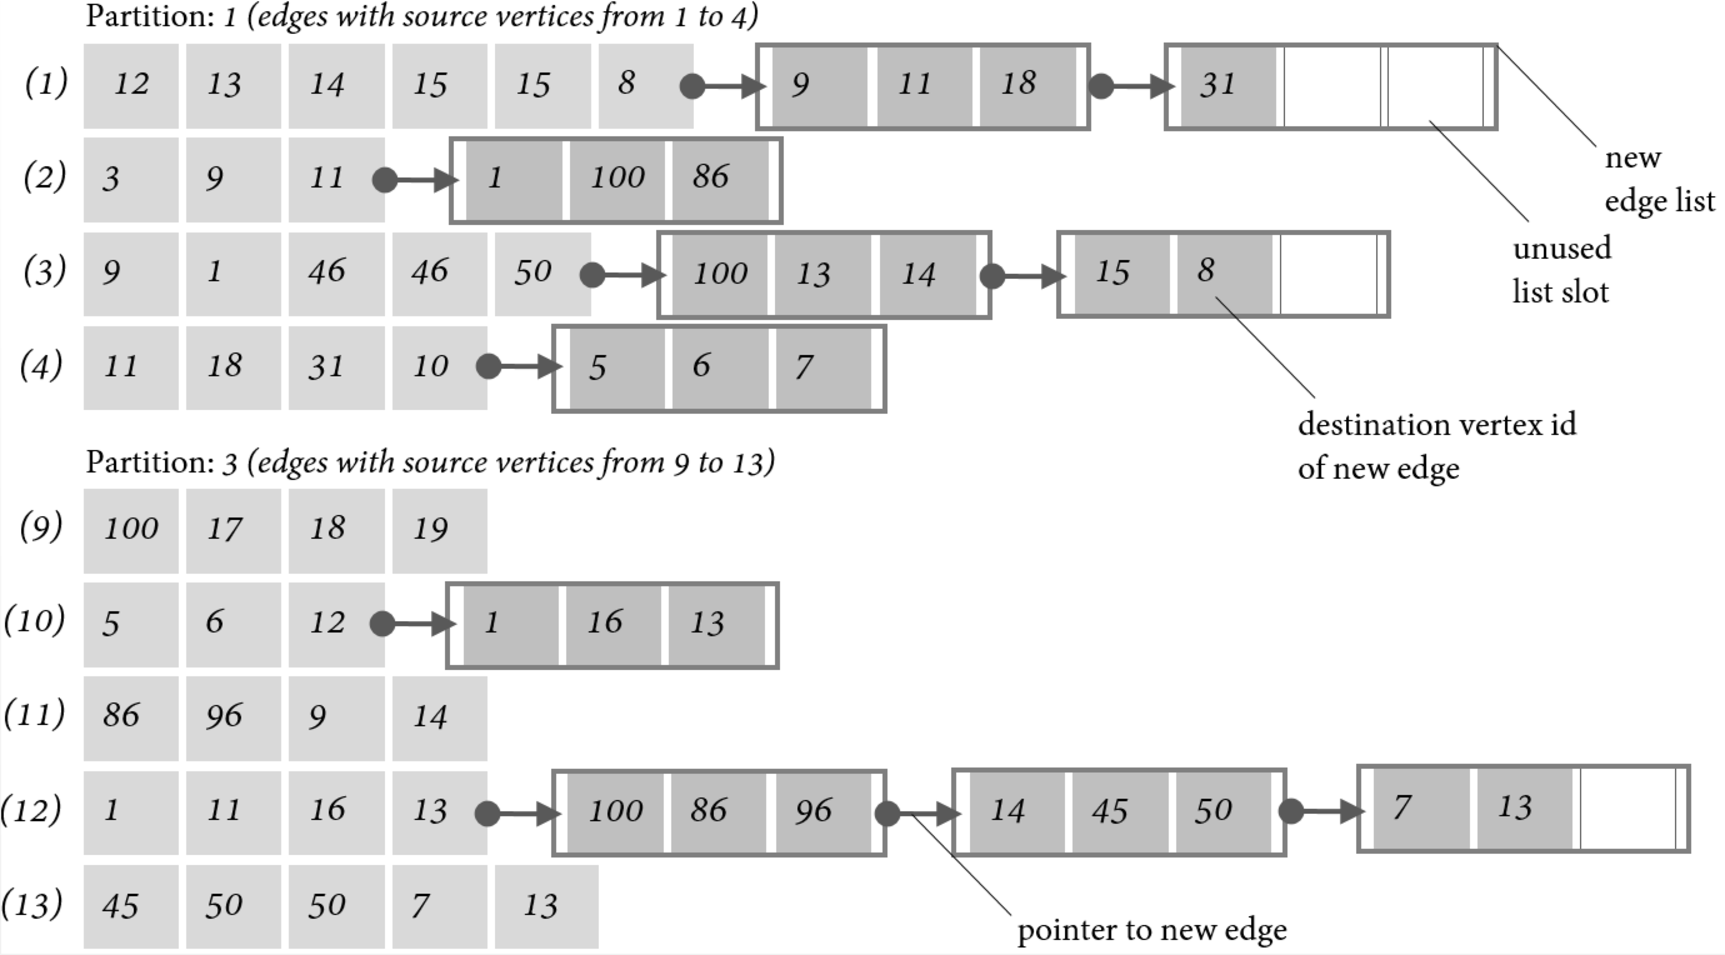
\includegraphics[scale=0.44]{Figures/newedgelsts.pdf}
	\end{center}
	\caption{Adjacency lists linked to new edge array lists of fixed sizes.}
	\label{fig-newedgelsts}
\end{figure*}

Fig.~\ref{fig-newedgelsts} shows how the newly computed edges are stored in the memory. As can be seen, the new edges are stored in a linked list, where each node of the linked list is an array. In order to refer to the linked lists we have used the \texttt{NewEdge-Lists} data structure as shown in Fig.~\ref{fig-newedgelstsencap}.

\begin{figure}[!htbp]
	\begin{center}
		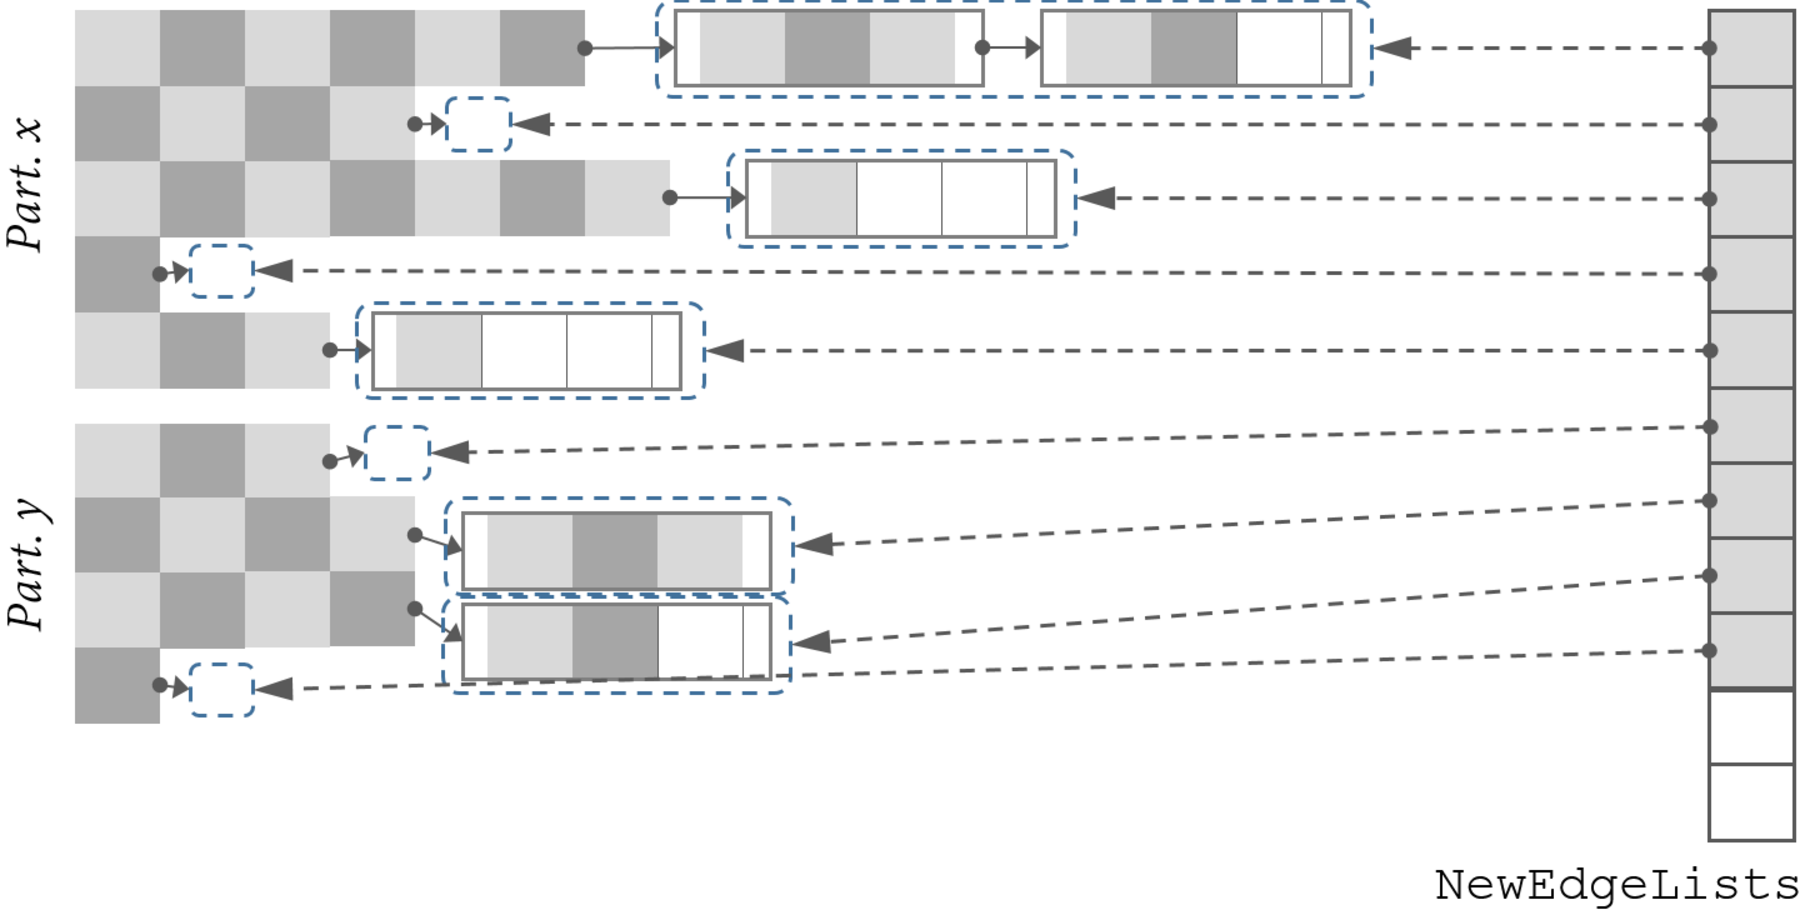
\includegraphics[scale=0.27]{Figures/newedgelstsencap.pdf}
	\end{center}
	\caption{NewEdgeLists data structure to refer to the newly computed edge lists of each loaded source vertex.}
	\label{fig-newedgelstsencap}
\end{figure}



We have used this storage design for new edges in order to obviate the need to declare new memory space every time a new edge is created, which is expensive considering the number of computations we will be dealing with. Instead we declare a new node only if an existing node is filled up. The drawback of this approach is that there may be some unused slots in these nodes. 

\begin{figure*}[!htbp]
	\begin{center}
		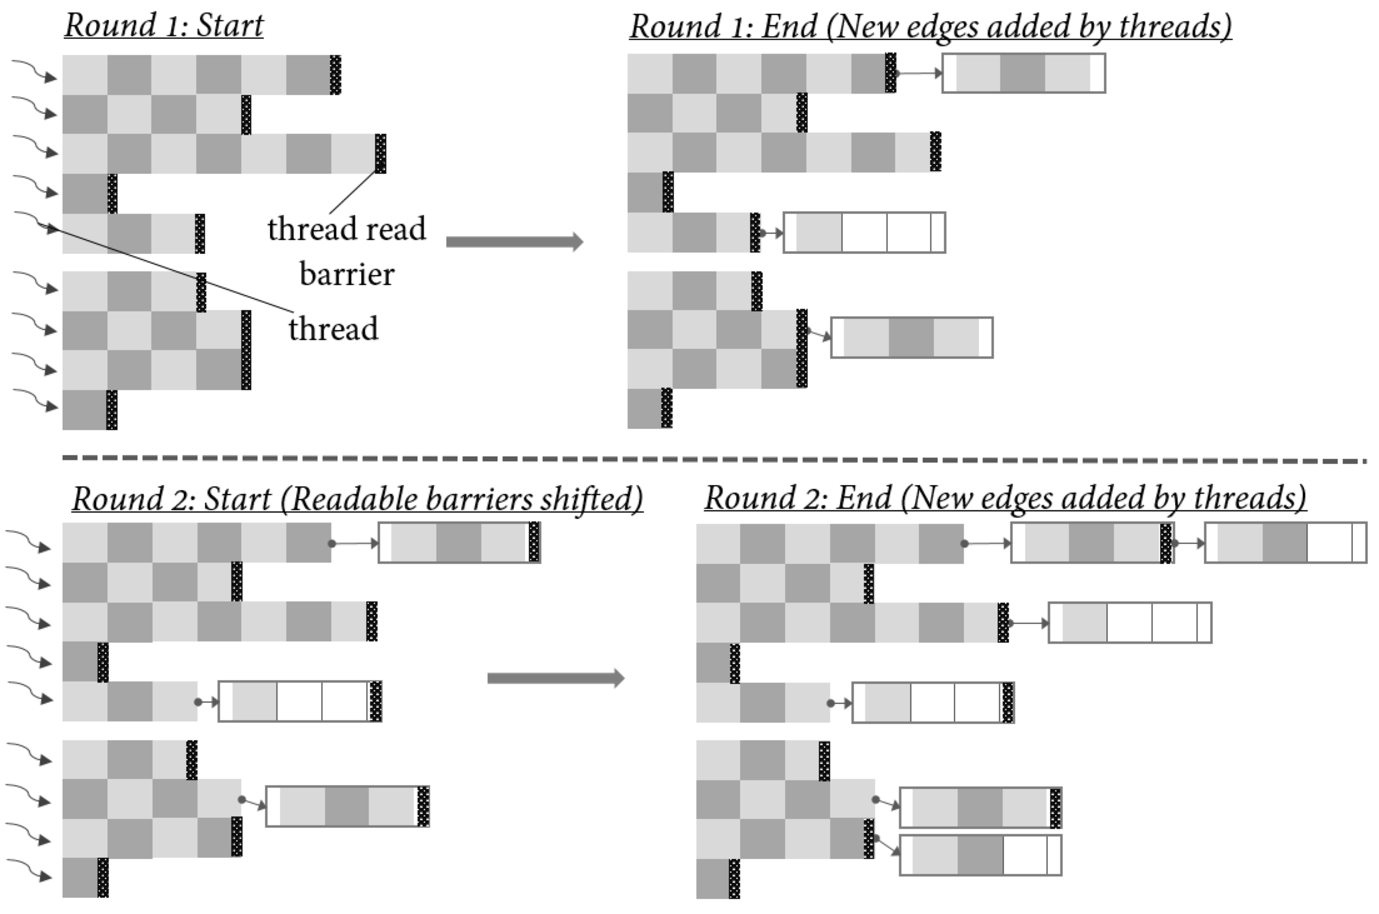
\includegraphics[scale=0.5]{Figures/multithrd1.pdf}
	\end{center}
	\caption{Multi-threaded edge computation design.}
	\label{fig-multithrd1}
\end{figure*}

Fig.~\ref{fig-multithrd1}, shows how the actual computations are carried out. As can be seen, we have used a multi-threaded design for the computation, where new edge computations for each source vertex row are done in-parallel. 

The process is carried out iteratively, wherein during each round, new edge computations are done based on the edges of the previous round. To facilitate this, we used readable barriers for each source vertex row. 

These barriers limit the extent of a source vertex row that can be read by a thread during a round. This consequently prevents a thread from reading an array slot that is being written on by another thread, which prevents atomicity issues. In order to know when a round has ended, we used an atomic integer variable. 

The atomic integer variable keeps a count of the number of active threads. Once it is 0, the computation proceeds to the next round, shifting the readable barriers ahead. The process repeats until no new edges have been generated in a particular round.

\begin{figure*}[!htbp]
	\begin{center}
		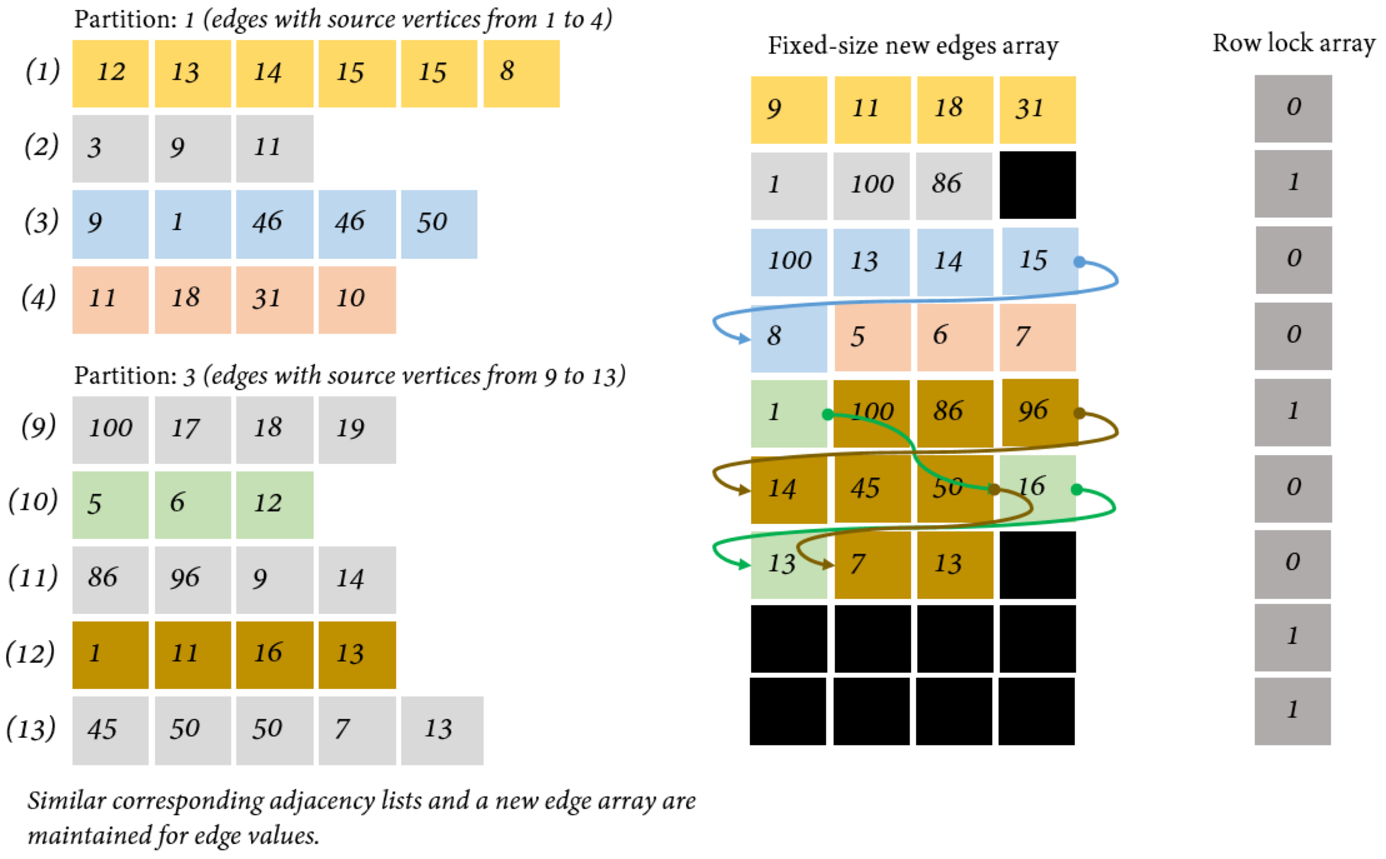
\includegraphics[scale=0.6]{Figures/alt.pdf}
	\end{center}
	\caption{Alternate design for edge computation.}
	\label{fig-alt}
\end{figure*} 

\textit{Alternate design for edge computation.} An alternate design for edge computation is shown in Fig.~\ref{fig-alt}. In this design, new edges are stored in a fixed-size multidimensional array, the size of which is declared at the beginning of the computation process. This approach eliminates the need to declare space for new edges completely, as it does so at the beginning. New edges are written in this array, and a table is used to record the correspondence between new edges and the loaded source vertex. The color coded cells in Fig.~\ref{fig-alt} illustrate this concept.

For parallelism, we use threads such that each thread accesses a synchronized row lock array. A thread begins to write on a row only if it has acquired a lock for that row. 

The problem with this technique is the maintenance of links. This is programmatically error prone as it requires consistent updating of ``new edges array'' indexes (first position, intermediate link positions, and last position) for each loaded source vertex. 

\subsection{Post Computation Processing}
\label{subsec:pcp}

The post-computation processing phase entails updating the vertex interval table, the degrees information, and the scheduling information, based on the new edges added. Although the process is inexpensive, it could be expensive if repartitioning is invoked on the partitions. We explain repartitioning next.

\subsection{Repartitioning}
\label{subsec:rprt}
Repartitioning is a sub-phase of post-computation processing which is invoked if the sizes of any of the loaded partitions go beyond a threshold limit. (Typically it is around a small percentage larger than the partition size). Like the post-computation processing phase, the repartitioning also involves updating the same in-memory data structures. However, the recalculation of scheduling information could bear the most cost if the scheduling metric mentioned in part~\ref{subsec:sch} is used for it would require scanning all the partitions once again. It is for this reason we want to keep the number of repartitionings in the entire execution of the graph to be minimum. For more details on scheduling cost see~\ref{subsec:sch}.

\subsection{Reloading}
\label{subsec:rld}

\begin{figure*}[!htbp]
	\begin{center}
		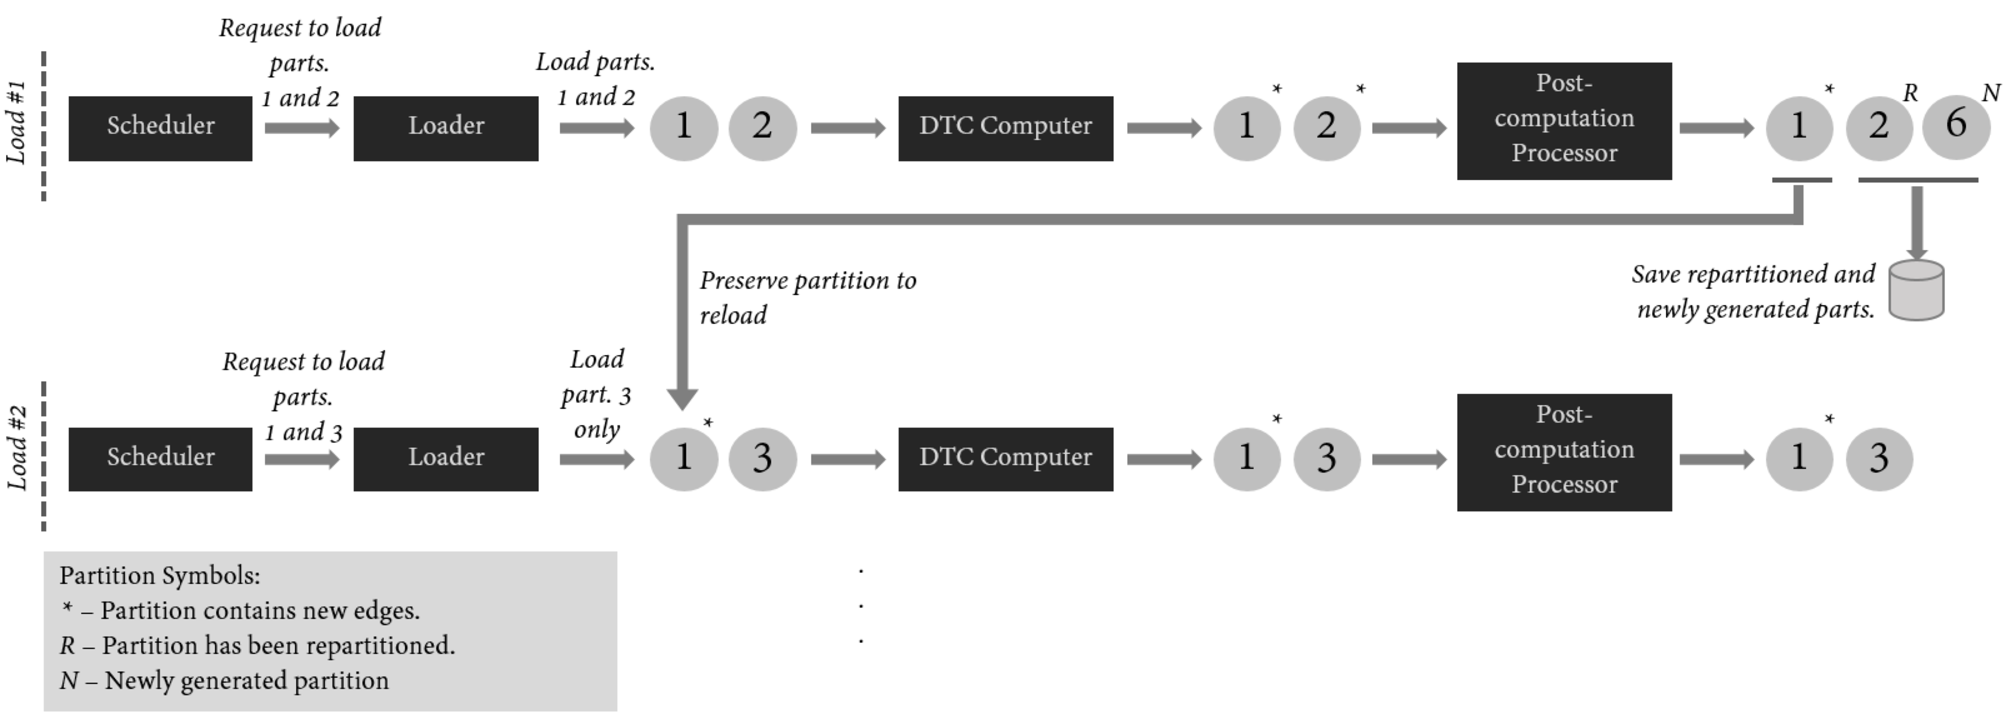
\includegraphics[scale=0.45]{Figures/partmgtdemo.pdf}
	\end{center}
	\caption{Example demonstrating in-memory partition management during GraphDTC execution.}
	\label{fig-partmgtdemo}
\end{figure*}

Although the main functionality of the reloading phase is the same as that of the loading phase, which is loading partitions, reloading also requires to preserve any of the loaded partitions in the memory if the partition is among the requested set of partitions for the next computation load. 

There could be a number of strategies for reloading. One such strategy is demonstrated in Fig.~\ref{fig-partmgtdemo}. With this strategy, partitions that have been repartitioned, and the new partitions that have been generated as a result, are saved directly in the disk and cleared from the memory, regardless of whether or not they are requested in the next round. An alternate and better strategy would be to hold all the partitions in the memory till the next load request is received from the scheduler. 

\subsection{Scheduling}
\label{subsec:sch}

The  design of the scheduling phase of GraphDTC is summed up in Fig.~\ref{fig-scheddsgn}. Scheduling in GraphDTC has two main objectives: (1) Maximize the number of edge pairs that form a path, and thus, that return a candidate new edge for checking, in a single load. (2) Favor the reuse of memory allocated for new edges during the previous load. 

For objective (1), the scheduler uses a metric known as the edge-destination count ratio, $X$, which is calculated for all possible pairs of partitions. So say, for partitions $P_a$ and $P_b$, $X_{({P_a},{P_b})}$ is the fraction of edges in partition $P_a$ that point to a vertex present in partition $P_b$ as a source vertex. A high $X$ value thus fulfills this objective. 

The scheduler uses a map of edge-destination count ratios and favors to pick the partition pair that has the highest value, during each iteration. Calculating this map requires scanning the entire graph (which is expensive), which was done during preprocessing. In order to update this map, we only need to scan the partitions to which new edges were added. However, scanning the entire graph becomes necessary if we want to update this map after repartitioning. 

For fulfilling objective (2), the scheduler only needs to know which partitions are currently loaded in the memory. 

Finally, apart from fulfilling these objectives, the scheduler also keeps track of the pairs of partitions that have been computed using the termination map. The purpose of this map is to avoid loading a partition-pair that has already been computed. It is important to note that during the computation of a partition-pair, if new edges were added, the computations of the other partitions with these partitions would again need to be performed. The termination map is updated according to this principle.

The scheduler continues to request the loader to load partitions at the conclusion of each computation iteration, until the termination map shows all existing partition pairs to be computed. 

\begin{figure}[!htbp]
	\begin{center}
		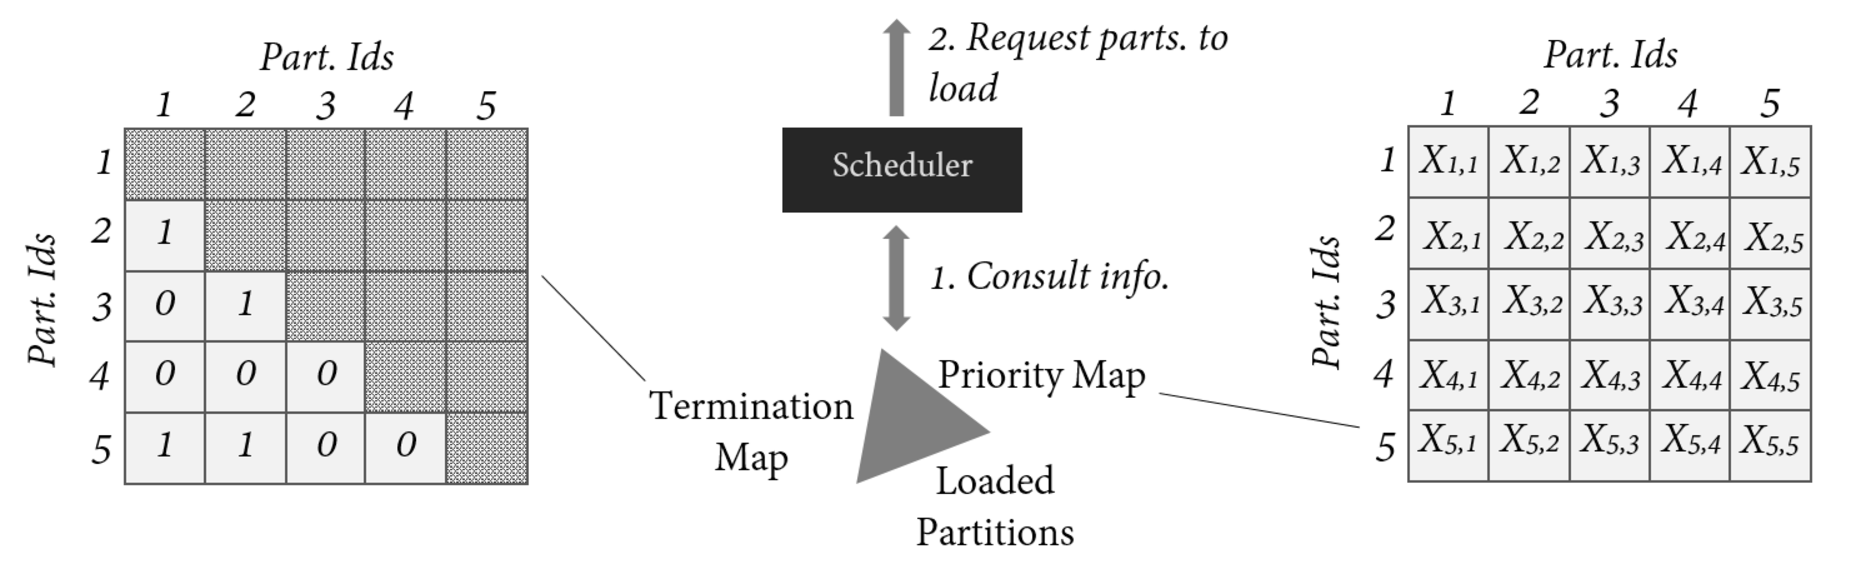
\includegraphics[scale=0.26]{Figures/scheddsgn.pdf}
	\end{center}
	\caption{Scheduler design for loading two partitions.}
	\label{fig-scheddsgn}
\end{figure}


%\subsection{Data Structures}
%\subsection{Performance Assessment}
\section{Evaluation Plan}
\label{sec:evpln}

In this section, we outline our plan for evaluating GraphDTC. We expect to perform the deployment required to fulfill these plans in a workstation supplanted with an Intel i5-4570 Processor, and 8GB of RAM.

The plan will be primarily driven by three objectives: (1) investigate the performance of GraphDTC when processing very large graphs (of the order of a billion vertices) (Subsection~\ref{subsec:lgperf}), (2) implement DTC with an existing graph processing system GraphChi~\cite{graphchi} and compare its results with ours (Subsection~\ref{subsec:gchicomp}), and finally (3) obtain the level of improvement that can be obtained when GraphDTC is used to leverage existing program analysis tools in terms of the reduction in false alarm rates (Subsection~\ref{subsec:leverpatools}). 

Based on the outcomes of our evaluation, we shall also intend to locate components of our system that are amenable for optimizations. 

\subsection{Performance with Large Graphs}
\label{subsec:lgperf}

We look to stress test our system with existing large graphs: the Yahoo Web Graph (6,636,600,779 edges, 67GB disk storage size) and the Twitter Social Graph (1,468,365,182 edges, 25GB disk storage size). In practice, these graphs are not the type of graphs that our system is meant to deal with. In fact, our system targets program graphs, which are expected to be large but much smaller than these graphs. Nevertheless, as our system is agnostic of the application domain of the graphs, doing these tests allows us to see how the system handles the pressure of performing computations on massive graphs. In addition, we expect these graphs to have varying structures. Therefore, processing them with our system allows us to verify more corner cases, and thus gain more confidence in our system's correctness. 

The only configuration parameter we shall need to change in our system for running it on the aforementioned graphs is to ignore edge labels, i.e. the grammar, and thus only compute basic transitive closure. 

\subsection{Comparison with GraphChi}
\label{subsec:gchicomp}

We intend to perform the DTC computation using a popular graph processing system, GraphChi~\cite{graphchi} and compare GraphDTC's performance with GraphChi's. 

Most distributed/parallel graph processing systems like Pregel~\cite{pregel}, Apache Giraph~\cite{giraph}, GraphLab~\cite{glab}, Kineograph~\cite{kg}, and also GraphChi, are built on the vertex centric model, where the user adopts the \textit{think-like-a-vertex (TLV)} approach to write applications on the system. Although this approach has been useful for writing algorithms involving propagation of vertex values (e.g. page-rank algorithm), we believe such an approach will increase the complexity and difficulty for writing applications for DTC computation. In particular, the edge matching process, which is easily achievable using the EPC model (shown in~\ref{subsec:epcm}), would be cumbersome to write using TLV. We also expect it to incur a significant performance overhead on GraphChi. 

\subsection{Leveraging Current Program Analysis Tools}
\label{subsec:leverpatools}

Towards leveraging program analysis tools we shall primarily target Coccinelle~\cite{Palix}. Coccinelle is a program matching and transformation tool that has been used to find faults in the kernel, drivers, and file systems of Linux. Our goal will be to increase the number of revealed true faults, and decrease the number of revealed false alarms, in Coccinelle. In order to do that, we shall first generate a call graph of Linux 2.6's kernel using LLVM~\cite{llvm}. Next, we plan to transform the graph to the prescribed input format of GraphDTC and perform the DTC operation on it. The resultant graph will carry more precise information, such as calling-context information, which we believe can benefit Coccinelle. 

%\section{Applications}
\label{sec:app}

%\section{Related Work}
\label{sec:rlwk}

\section{Conclusion}
\label{sec:cncl}

In this technical report, we have presented a graph processing system, GraphDTC, that can efficiently compute dynamic transitive closure (DTC) on program graphs of large complex systems, using a single machine. Consequently, the system can benefit static program analysis tools, that are today extensively used for revealing various diagnostic information of software programs. The novelty of GraphDTC lies in the fact that it provides a systems solution to the precision-efficiency bottleneck of software analysis, by addressing a fundamental problem in programming language design, the CFL-reachability problem. The technical report also elaborates upon an evaluation plan for the system.

\bibliographystyle{acm}
\bibliography{biblio}

\end{document}